\documentclass[aspectratio=169,10pt]{beamer}
\usetheme{Madrid}
\usecolortheme{default}
\usepackage[utf8]{inputenc}
\usepackage[T1]{fontenc}
\usepackage{amsmath,amssymb,bm,booktabs,graphicx,tikz}
\usetikzlibrary{arrows.meta,positioning,calc}
\setbeamertemplate{navigation symbols}{}
\setbeamertemplate{footline}[frame number]

% ---------- macros ----------
\newenvironment{psmallmatrix}{\left(\begin{smallmatrix}}{\end{smallmatrix}\right)}
\newcommand{\R}{\mathbb{R}}
\newcommand{\tr}{\operatorname{tr}}
\newcommand{\sgn}{\operatorname{sign}}
\newcommand{\lmin}{\lambda_{\min}}
\newcommand{\lmax}{\lambda_{\max}}
\newcommand{\dq}{\dot q}
\newcommand{\Wt}{\tilde W}
\newcommand{\Dt}{\tilde\Delta}
\newcommand{\norm}[1]{\left\lVert #1\right\rVert}
\newcommand{\placeholder}[2]{%
  \begin{center}\fbox{\parbox[c][#2][c]{0.85\textwidth}{\centering\large\textit{#1}}}\end{center}}

\title[PBC + Structured Learning]{Passivity-Based Control with Physics-Informed\\Structured Learning for Robot Manipulators}
\subtitle{Progress report}
\author{José Aarón Barbosa Mercado}
\institute[CINVESTAV]{CINVESTAV-IPN\\[2pt]\small Advisors: Dr.\ Wen Yu Liu \;\&\; Dr.\ Fernando Castaños Luna}
\date{}

\begin{document}

\begin{frame}\titlepage\end{frame}

\begin{frame}{Outline}
\begin{enumerate}\setlength\itemsep{3pt}
\item Problem and architecture
\item Nominal model of the 2R manipulator
\item Slotine--Li and the passivity template (Ortega--Spong)
\item Passivity, feedback equivalence, global stabilization (Byrnes--Isidori--Willems)
\item Nominal passivity-based controller and baseline radius
\item DeLaN and its role; span extension
\item Integral-momentum regression (acceleration-free)
\item Spectral normalization and the Lipschitz certificate
\item Online learning law: passivity derivations and robust modification
\item Super-twisting action and the composite Lyapunov function
\item Simulation results, open points, next steps
\end{enumerate}
\end{frame}

%==================================================================
\section{Problem and architecture}
\begin{frame}{Problem statement}
Fully actuated manipulator, Euler--Lagrange model
\[
M(q)\ddot q + C(q,\dq)\dq + g(q) + F(\dq) + \tau_d = \tau .
\]
\textbf{Structural properties} (used throughout):
\begin{itemize}
\item $\lambda_m I \le M(q)\le \lambda_M I$, \quad $\dot M = C + C^\top$ (Christoffel) $\Rightarrow x^\top(\dot M-2C)x=0$
\item $\dq^\top F(\dq)\ge 0$ (dissipative friction), growth bounds on $C,g$
\end{itemize}
\textbf{Goal:} track $q_d(t)$ despite unknown $M,C,g,F,\tau_d$, with:
\begin{enumerate}
\item a nominal model giving a \emph{guaranteed} baseline error radius,
\item a structured learning module that shrinks the residual while \emph{preserving} the physics,
\item a robust (super-twisting) action for what remains,
\item a stability argument that is \emph{modular}: each block certified through passivity.
\end{enumerate}
\end{frame}

\begin{frame}{Architecture}
\begin{center}
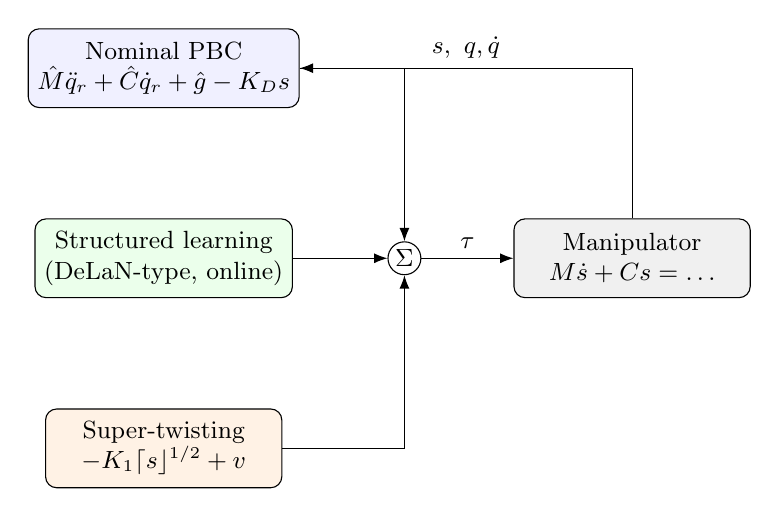
\begin{tikzpicture}[node distance=14mm and 18mm, every node/.style={font=\small},
 blk/.style={draw,rounded corners,minimum width=30mm,minimum height=10mm,align=center,fill=blue!6}]
\node[blk] (pbc) {Nominal PBC\\$\hat M\ddot q_r+\hat C\dq_r+\hat g-K_Ds$};
\node[blk,below=of pbc,fill=green!8] (nn) {Structured learning\\(DeLaN-type, online)};
\node[blk,below=of nn,fill=orange!10] (sta) {Super-twisting\\$-K_1\lceil s\rfloor^{1/2}+v$};
\node[blk,right=28mm of nn,fill=gray!12] (plant) {Manipulator\\$M\dot s+Cs=\ldots$};
\node[circle,draw,inner sep=1pt,right=12mm of nn] (sum) {$\Sigma$};
\draw[-Latex] (pbc.east) -| (sum.north);
\draw[-Latex] (nn.east) -- (sum.west);
\draw[-Latex] (sta.east) -| (sum.south);
\draw[-Latex] (sum.east) -- node[above]{$\tau$} (plant.west);
\draw[-Latex] (plant.north) |- node[above,pos=0.75]{$s,\ q,\dq$} (pbc.east);
\end{tikzpicture}
\end{center}
\vspace{-2mm}
\small Sliding variable $s=\dot e+\Lambda e$, $\ e=q-q_d$; reference $\dq_r=\dq_d-\Lambda e$, $\ \ddot q_r$ its derivative.
\end{frame}

\begin{frame}{The modularity argument}
\begin{itemize}
\item Adding a weight term to a quadratic storage is \emph{not} unique to passivity (standard adaptive control does it).
\item What passivity buys: each block is certified through its own \emph{port} map; the negative feedback of passive systems is passive.
\item With the interconnection fixed, \textbf{swapping a module only requires re-certifying that module's passivity} (e.g.\ another learner, another robust term).
\item In this thesis the modules are chosen (PBC, DeLaN-type learner, STA), so the immediate benefit is a clean certificate and a physical interpretation of what each block contributes.
\end{itemize}
\vspace{2mm}
\begin{block}{Caveat}
The STA is \emph{not} passive in the quadratic sense; that block is certified differently.
\end{block}
\end{frame}

%==================================================================
\section{Nominal model: 2R planar arm}
\begin{frame}{2R planar manipulator: results}
Parameters $m_i,\ l_i,\ l_{c_i},\ I_i$; $\;c_{12}=\cos(q_1+q_2)$, $h=m_2l_1l_{c_2}\sin q_2$.
\[
M(q)=\begin{pmatrix}
m_1l_{c_1}^2+m_2(l_1^2+l_{c_2}^2+2l_1l_{c_2}\cos q_2)+I_1+I_2 & m_2(l_{c_2}^2+l_1l_{c_2}\cos q_2)+I_2\\
m_2(l_{c_2}^2+l_1l_{c_2}\cos q_2)+I_2 & m_2l_{c_2}^2+I_2
\end{pmatrix}
\]
\[
C(q,\dq)=\begin{pmatrix}-h\dq_2 & h\dq_1\\ -h\dq_1-h\dq_2 & 0\end{pmatrix},\qquad
g(q)=\begin{pmatrix}(m_1l_{c_1}+m_2l_1)g\cos q_1+m_2gl_{c_2}\cos q_{12}\\ m_2gl_{c_2}\cos q_{12}\end{pmatrix}
\]
\small
\begin{itemize}
\item Only $q_2$ enters $M$; $C$ from Christoffel symbols; $g=\nabla_q P$ with $P=m_1gl_{c_1}\sin q_1+m_2g(l_1\sin q_1+l_{c_2}\sin q_{12})$.
\item Checked: $\dot M=C+C^\top$ (skew-symmetry of $\dot M-2C$).
\item End effector: $x=l_1\cos q_1+l_2\cos q_{12}$, $y=l_1\sin q_1+l_2\sin q_{12}$.
\end{itemize}
\end{frame}

%==================================================================
\section{Slotine--Li and the passivity template}
\begin{frame}{Slotine--Li: the baseline approach}
\textbf{Reference signals:} $s=\dot e+\Lambda e=\dq-\dq_r$, $\ \dq_r=\dq_d-\Lambda e$.\\[2mm]
\textbf{Linear parametrization:} $M\ddot q+C\dq+g=Y(q,\dq,\ddot q)\,\theta$.\\[2mm]
\textbf{Control:} $\tau=Y(q,\dq,\dq_r,\ddot q_r )\hat\theta-K_Ds$. With $\tilde\theta=\hat\theta-\theta$:
\[
M\dot s+Cs=Y\tilde\theta-K_Ds .
\]
\textbf{Lyapunov:} $V=\tfrac12 s^\top Ms+\tfrac12\tilde\theta^\top\Gamma^{-1}\tilde\theta$,
\[
\dot V=-s^\top K_Ds+\tilde\theta^\top\!\big(Y^\top s+\Gamma^{-1}\dot{\hat\theta}\big)
\;\overset{\dot{\hat\theta}=-\Gamma Y^\top s}{=}\;-s^\top K_Ds\le0 .
\]
Barbalat: $s\in\mathcal L_2\cap\mathcal L_\infty$, $\dot s\in\mathcal L_\infty\Rightarrow s\to0\Rightarrow e,\dot e\to0$.\\[1mm]
\textbf{Limitation:} needs an exact linear-in-parameters structure (no unmodelled dynamics) $\Rightarrow$ motivates the \emph{learned} residual.
\end{frame}

\begin{frame}{Ortega--Spong: passivity as the unifying template}
\begin{itemize}
\item Error system: $\;-\Psi\ (\text{identification/regressor error})\ \to\ r$ is passive; the adaptation law is a passive map $r\to\Psi$.
\item \textbf{Theorem 3 (Ortega--Spong '89):} negative feedback of the passive dynamics map and the passive adaptation map gives boundedness and convergence of $r$.
\item Slotine--Li is the special case $K(s)=\Lambda/s$, i.e.\ $r=F(s)^{-1}e$ with $F$ strictly proper stable.
\end{itemize}
\vspace{1mm}
\begin{center}
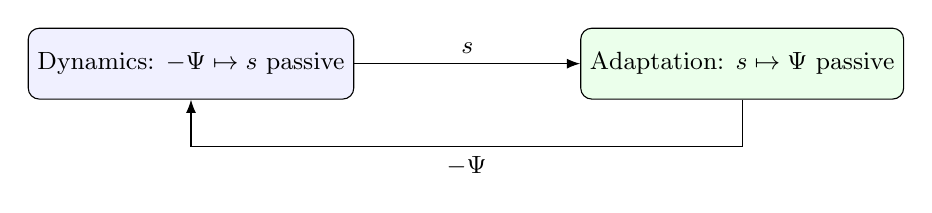
\begin{tikzpicture}[font=\small,blk/.style={draw,rounded corners,minimum width=34mm,minimum height=9mm,align=center}]
\node[blk,fill=blue!6] (A) at (0,0) {Dynamics: $-\Psi\mapsto s$ passive};
\node[blk,fill=green!8] (B) at (7,0) {Adaptation: $s\mapsto\Psi$ passive};
\draw[-Latex] (A.east) -- node[above]{$s$} (B.west);
\draw[-Latex] (B.south) -- ++(0,-6mm) -| node[below,pos=0.25]{$-\Psi$} (A.south);
\end{tikzpicture}
\end{center}
\textbf{In this thesis:} same template, but $\Psi=\tilde\Delta$ (residual) and the passive adaptation block is the output-layer law of a structured network.
\end{frame}

%==================================================================
\section{Passivity theory}
\begin{frame}{Dissipativity and passivity (Byrnes--Isidori--Willems)}
$\dot x=f(x)+g(x)u,\ \ y=h(x)$. Supply rate $w=u^\top y$.
\begin{itemize}
\item \textbf{Passive:} $\exists\,S\ge0$: $S(x(t))\le S(x(0))+\int_0^tu^\top y$ \quad($\dot S\le u^\top y$).
\item \textbf{Lossless:} equality. \textbf{OSP:} extra $-\epsilon\|y\|^2$. \textbf{ISP:} extra $-\delta\|u\|^2$.
\item \textbf{Available storage} $S_a(x)=\sup\int_0^T -u^\top y$; finite $\iff$ dissipative; with reachability, $S_a$ is a storage.
\item \textbf{KYP property:} $L_fS\le0$, $\ L_gS=h^\top$. For smooth storage, equivalent to passivity: it is the differential form of $\dot S\le u^\top y$ holding for \emph{all} $u$.
\item \textbf{Zero-state detectability + output feedback} $u=-\phi(y)$, $y^\top\phi(y)>0$: asymptotic stability (LaSalle); global if $S$ is proper.
\end{itemize}
\end{frame}

\begin{frame}{Relative degree, normal form, minimum phase}
\begin{itemize}
\item \textbf{Relative degree one:} $L_gh(x)$ invertible; $\dot y=L_fh+L_gh\,u$ (linear: $\deg(\text{den})-\deg(\text{num})=1$).
\item \textbf{Normal form:} coordinates $(z,y)$:
\[\dot z=q(z,y),\qquad \dot y=a(z,y)+b(z,y)u .\]
\item \textbf{Zero dynamics:} $\dot z=q(z,0)$ (internal dynamics when $y\equiv0$).
\item \textbf{Minimum phase:} zero dynamics asymptotically stable (linear: stable inverse). \textbf{Weakly minimum phase:} Lyapunov-stable with a $C^2$ function $W$, $L_{q}W\le0$.
\end{itemize}
\begin{block}{Manipulator ($y=\dq$)}
$\dot y=M^{-1}(\tau-\dots)$: relative degree one. Zero dynamics: $\dq\equiv0$, $q=$ const (every point an equilibrium) $\Rightarrow$ \emph{weakly} minimum phase. Energy $H=\tfrac12\dq^\top M\dq+U$ gives $\dot H=\dq^\top\tau-\dq^\top F\le\dq^\top\tau$.
\end{block}
\end{frame}

\begin{frame}{Feedback equivalence and stabilization}
\begin{theorem}[BIW 1991]
(i) A passive system with a $C^2$ positive definite storage has relative degree one (if $\operatorname{rank}g(0)=m$) and is weakly minimum phase. (ii) Locally, a system is feedback equivalent ($u=\alpha(x)+\beta(x)v$) to a passive system with $C^2$ positive definite storage iff it has relative degree one and is weakly minimum phase.
\end{theorem}
\begin{itemize}
\item Consequence: for such systems, $v=-\phi(y)$ plus zero-state detectability gives asymptotic stabilization; with global versions of the hypotheses and proper storage, \textbf{global} stabilization.
\item Cascade view (Thm.\ 5.1): if the $y$-subsystem is stabilized and the zero dynamics are (weakly) stable, the cascade is stabilized.
\end{itemize}
\textbf{Relevance:} the manipulator is already passive from $\tau$ to $\dq$; the sliding variable $s=\dot e+\Lambda e$ is the passive output that adds convergence of $e$ (filtering of a passive output through a stable minimum-phase filter).
\end{frame}

%==================================================================
\section{Nominal PBC and baseline radius}
\begin{frame}{Nominal passivity-based controller}
\[
\tau=\hat M\ddot q_r+\hat{C}\dq_r+\hat g-K_Ds\;(+\hat\Delta_{\text{learned}}+\tau_{sta}).
\]
Define the uncertainty $\Delta=(M-\hat M)\ddot q_r+(C-\hat C)\dq_r+(g-\hat g)+F+\tau_d$ and $\tilde\Delta=\Delta-\hat\Delta$:
\[
M\dot s=-Cs-K_Ds-\tilde\Delta .
\]
With $V=\tfrac12 s^\top Ms$:
\[
\dot V=-\tfrac12s^\top(\dot M-2C)s-s^\top K_Ds-s^\top\tilde\Delta=-s^\top K_Ds-s^\top\tilde\Delta .
\]
\begin{block}{Passivity certificate}
$-\tilde\Delta\to s$ is \textbf{output strictly passive} with storage $V$ and rate $\lmin(K_D)$.\\
Nominal-only: $\hat\Delta=0$, so $\tilde\Delta=\Delta$.
\end{block}
\end{frame}

\begin{frame}{Baseline radius}
Young with $\Lambda_1\succ0$: $-s^\top\Delta\le s^\top\Lambda_1s+\tfrac14\Delta^\top\Lambda_1^{-1}\Delta$, so
\[
\dot V\le-s^\top(K_D-\Lambda_1)s+\bar\eta_1\le-\alpha V+\bar\eta_1,\quad
\alpha=\frac{2\lmin(K_D-\Lambda_1)}{\lambda_M},\ \ \bar\eta_1=\sup_t\tfrac14\Delta^\top\Lambda_1^{-1}\Delta .
\]
Comparison lemma $\Rightarrow$ ultimate bound
\[
\boxed{\ \limsup\|s\|\le\rho_1=\sqrt{\frac{\bar\eta_1\,\lambda_M}{\lmin(K_D-\Lambda_1)\,\lambda_m}}\ }
\]
and $e,\dot e$ bounded through the stable filter $s=\dot e+\Lambda e$.
\begin{itemize}
\item Larger $K_D$ $\Rightarrow$ smaller $\rho_1$ (confirmed in the sandbox).
\item $\bar\eta_1$ is the quantity the learning module is meant to reduce.
\end{itemize}
\end{frame}

\begin{frame}{Sandbox: nominal PBC with unmatched dynamics}
\begin{columns}[c]
\begin{column}{0.58\textwidth}
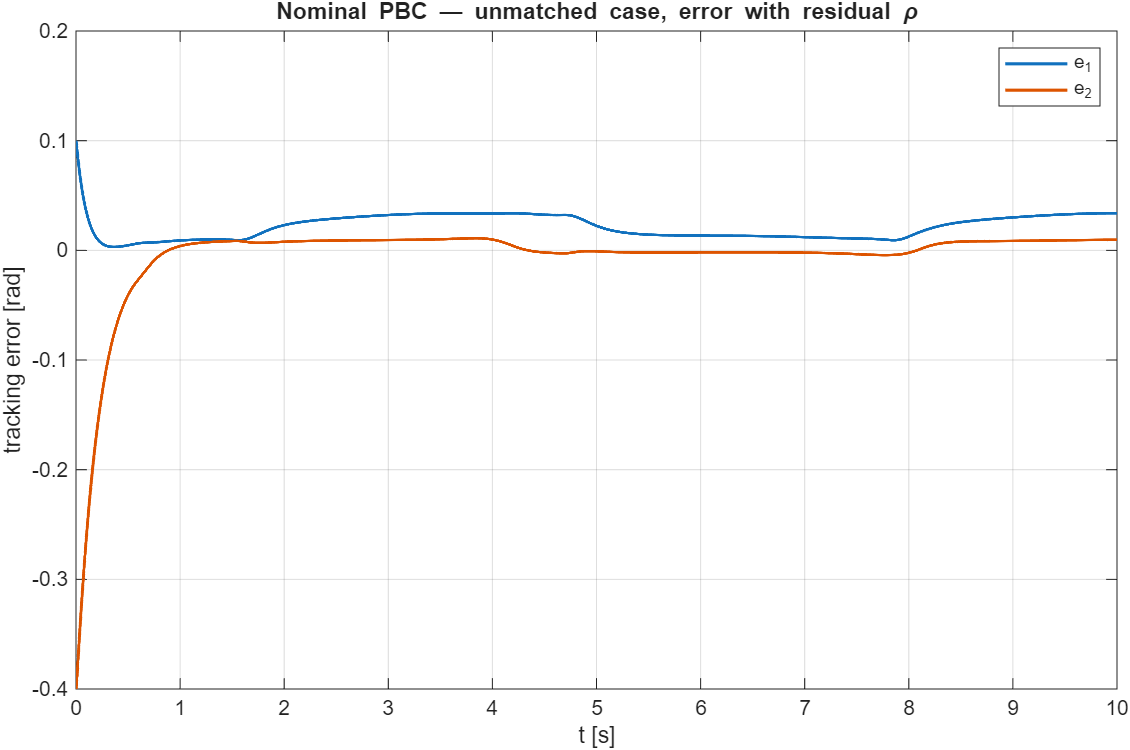
\includegraphics[width=\textwidth]{Images/pbc_unmatched.png}
\end{column}
\begin{column}{0.4\textwidth}
\small
\textbf{Setup:} plant with $m_2\times1.2$, $l_{c_2}\times0.9$ plus joint friction; controller uses the nominal values. $K_D=20$.
\begin{itemize}
\item Error stays in a bounded band (below $\sim$0.02\,rad).
\item Radius grows as $K_D$ decreases.
\item Bumps coincide with $\dq_1=0$ (Stribeck friction).
\item Friction smoothed with $\tanh(\dq/0.01)$.
\end{itemize}
\end{column}
\end{columns}
\end{frame}

%==================================================================
\section{DeLaN}
\begin{frame}{DeLaN: physics-informed structured learning}
Lagrangian $\mathcal L=\tfrac12\dq^\top M(q)\dq-U(q)$; Euler--Lagrange gives $M\ddot q+C\dq+\nabla U=\tau$. Only $M$ and $U$ need to be learned:
\begin{itemize}
\item $\hat M=\hat L(q;\theta)\hat L^\top(q;\theta)+\epsilon I$, $\ \hat L$ lower triangular, non-negative diagonal $\Rightarrow\hat M\succeq\epsilon I$.
\item $\hat C$ from $\hat M$ via Christoffel symbols $\Rightarrow\dot{\hat M}-2\hat C$ skew by construction.
\item $\hat g=\nabla_q\hat U(q;\psi)$ via automatic differentiation.
\item Friction: monotone activations + non-negative weights $\Rightarrow\dq^\top\hat F\ge0$.
\end{itemize}
Original DeLaN: offline unsupervised/supervised fit of the decomposition.\\[1mm]
\textbf{Role here:} supplies \emph{structure-preserving features}. Offline: learn the basis; online: only the output layer adapts (linear in weights) with a Lyapunov law $\Rightarrow$ the learning block remains passive.
\end{frame}

\begin{frame}{Thesis extension: conic combination of frozen bases}
Problem: with a single frozen $\bar L$, scalar gains reach only multiples of $\bar L\bar L^\top$ (e.g.\ $\begin{psmallmatrix}4&2\\2&4\end{psmallmatrix}$ but never $\begin{psmallmatrix}4&1\\1&4\end{psmallmatrix}$).\\[1mm]
\textbf{Fix:} $k$ frozen factors $\bar L_j$ and non-negative weights
\[
\hat M_\omega(q)=\sum_{j=1}^k\omega_j\,\bar L_j(q)\bar L_j(q)^\top+\epsilon I,\quad\omega_j\ge0 .
\]
\begin{itemize}
\item PSD and $\ge\epsilon I$ for \emph{every} $\omega$ in the cone: structure cannot be destroyed online.
\item Any PSD matrix is a conic combination of rank-one projectors $\Rightarrow$ with rich enough $\bar L_j$ the span is not a restriction.
\item $\hat C$ is linear in $\hat M$ (Christoffel is linear), hence slaved to the same weights.
\item Gravity channel: weights of free sign (potential field).
\item Projection onto the convex cone preserves $\dot V$ (since $W^*\in\mathcal W$ convex): $\tr\{\tilde W^\top(\operatorname{Proj}(\cdot)-\cdot)\}\le0$.
\end{itemize}
Residual from limited span is lumped into $\varepsilon$ (approximation error).
\end{frame}

%==================================================================
\section{Integral momentum regression}
\begin{frame}{Acceleration-free regression: integral momentum}
Momentum $p=M\dq$ and $\dot M=C+C^\top$:
\[
\frac{d}{dt}(M\dq)=M\ddot q+\dot M\dq=\tau-g-F+C^\top\dq .
\]
Integrate over a window $[t_1,t_2]$ (no $\ddot q$ needed):
\[
\boxed{\ M(q_2)\dq_2-M(q_1)\dq_1=\int_{t_1}^{t_2}\!\big[\tau-g(q)-F(\dq)+C^\top(q,\dq)\dq\big]dt\ }
\]
\begin{itemize}
\item Regression targets from measured $q,\dq,\tau$ only; integration acts as a low-pass filter.
\item Data: Fourier-series excitation trajectories (Swevers et al.\ 1997) $\to$ persistent excitation / coverage of the workspace.
\item Pipeline implemented in the sandbox: excitation $\to$ simulated data $\to$ windowed momentum samples; identity verified with the true parameters.
\item Identity from De Luca \& Mattone (generalized momenta).
\end{itemize}
\end{frame}

%==================================================================
\section{Spectral normalization}
\begin{frame}{Spectral normalization and the Lipschitz constant}
For a feedforward network $f=W^{L+1}\sigma(\cdots\sigma(W^1x))$ with $\sigma$ 1-Lipschitz:
\[
\|f\|_{\mathrm{Lip}}\le\prod_l\sigma_{\max}(W^l).
\]
\textbf{Normalization (Miyato '18; Neural Lander):}
\[
\bar W^l=\frac{W^l}{\sigma_{\max}(W^l)}\,\gamma^{1/(L+1)}\ \Rightarrow\ \|f\|_{\mathrm{Lip}}\le\gamma .
\]
($\sigma_{\max}$ = largest singular value, \emph{not} the activation; power iteration.)
\begin{itemize}
\item $\gamma$ is a design parameter: lower bound from approximation capacity (error $\varepsilon$), upper bound from the stability conditions.
\item Neural Lander use: Lipschitz bound on $f(x_1)-f(x_2)$ in the Lyapunov derivative ($\lmin(K_v)>L_a\rho$) and, secondarily, training stability.
\item \textbf{Our use differs:} a bound on $\|\dot{\tilde\Delta}\|$ for the STA (next slides).
\end{itemize}
\end{frame}

\begin{frame}{What the Lipschitz certificate is needed for}
Without STA: the weight bound (e-mod) and the $\mathcal L_2$/UUB certificate already hold; \textbf{no Lipschitz constant needed}.\\[1mm]
With STA: need $\|\dot{\tilde\Delta}\|\le L_\theta$. Three contributions:
\begin{enumerate}
\item plant growth (through $M,C,g$ bounds and $\ddot q_r$),
\item network Jacobian: $\dfrac{\partial\Sigma}{\partial x}\dot x$, bounded via spectral normalization,
\item adaptation rate $\|\dot{\hat W}\|$ (bounded by the law and weight bounds).
\end{enumerate}
\begin{alertblock}{Open point}
Coriolis and gravity channels are first derivatives of networks, so their \emph{time} derivative needs \textbf{second}-derivative bounds (smooth activations). Spectral normalization alone only controls first-order Lipschitz for the inertia-type output channel.
\end{alertblock}
\end{frame}

%==================================================================
\section{Online learning law}
\begin{frame}{Learning law: exact cancellation}
Network output layer: $\hat\Delta=\hat W\Sigma(x)$, $\ \Delta=W^*\Sigma+\varepsilon$, $\ \tilde W=\hat W-W^*$, so $\tilde\Delta=\varepsilon-\tilde W\Sigma$.\\[1mm]
$V_\ell=\tfrac12s^\top Ms+\tfrac12\tr\{\tilde W^\top K_w^{-1}\tilde W\}$:
\[
\dot V_\ell=-s^\top K_Ds-s^\top\varepsilon+\tr\{\tilde W^\top(s\Sigma^\top+K_w^{-1}\dot{\hat W})\}
\]
using $s^\top\tilde W\Sigma=\tr\{\tilde W^\top s\Sigma^\top\}$ (cyclic invariance; the derivative passes inside the linear trace). Choose
\[
\boxed{\ \dot{\hat W}=-K_w\,s\,\Sigma^\top\ }\quad(\text{projected onto }\mathcal W)\ \Rightarrow\ \dot V_\ell=-s^\top K_Ds-s^\top\varepsilon .
\]
\begin{itemize}
\item \textbf{Which dynamics?} The error dynamics with the \emph{residual}: $\tilde\Delta=\varepsilon-\tilde W\Sigma$ (the $W^*\Sigma$ part is what is being learned).
\end{itemize}
\end{frame}

\begin{frame}{Passivity of the learning module and $\mathcal L_2$ gain}
Input $u=-\varepsilon$, output $y=s$:
\[
\dot V_\ell=u^\top y-y^\top K_Dy\le u^\top y-\rho\|y\|^2,\qquad\rho=\lmin(K_D)
\]
$\Rightarrow$ \textbf{output strictly passive} ($-\varepsilon\to s$). Young: $u^\top y\le\frac1{2\rho}\|u\|^2+\frac\rho2\|y\|^2$:
\[
\dot V_\ell\le\tfrac1{2\rho}\|u\|^2-\tfrac\rho2\|y\|^2
\ \Rightarrow\ \|s\|_2^2\le\tfrac2\rho V_\ell(0)+\tfrac1{\rho^2}\|\varepsilon\|_2^2 ,
\]
\[
\boxed{\ \|s\|_2\le\sqrt{\tfrac{2V_\ell(0)}{\rho}}+\tfrac1\rho\|\varepsilon\|_2\ }\qquad(\varepsilon\in\mathcal L_2).
\]
\begin{itemize}
\item Bad learning degrades performance but does not compromise stability.
\item Interconnection: the PBC block ($-\tilde\Delta\to s$) and the learner ($-\varepsilon\to s$) are two views of the \emph{same} port; only the storage/input definition changes, the output $s$ is shared.
\end{itemize}
\end{frame}

\begin{frame}{Robust modification (e-modification)}
\[
\dot{\hat W}=-K_w\big[s\Sigma^\top+\kappa\|s\|\hat W\big],\quad\kappa>0 .
\]
Extra term: $-\kappa\|s\|\langle\tilde W,\hat W\rangle_F$ with $\hat W=\tilde W+W^*$. Using Cauchy--Schwarz and completing the square,
\[
\langle W^*,\hat W\rangle_F-\|\hat W\|_F^2\le-\big(\|\hat W\|_F-\tfrac12\|W^*\|_F\big)^2+\tfrac14\|W^*\|_F^2 ,
\]
so
\[
\dot V_\ell\le-\lmin(K_D)\|s\|^2+\tfrac\kappa4\|W^*\|_F^2\|s\|+s^\top(\tau_{sta}-\varepsilon).
\]
\begin{itemize}
\item Ultimate bound (no STA): $\ \|s\|\lesssim\sqrt{\tfrac{\lambda_M}{\lambda_m}}\,\dfrac{\frac\kappa4\|W^*\|_F^2+\bar\varepsilon}{\lmin(K_D)}$, weights bounded (projection).
\item \textbf{Passivity status:} bias linear in $\|s\|$, so \emph{not} OSP; it is \textbf{semi-passive} (Pogromsky): dissipative outside a ball whose radius is set by $\kappa\|W^*\|_F^2$.
\item Trade-off: larger $\kappa$ $\Rightarrow$ stronger drift protection, larger ball.
\end{itemize}
\end{frame}

%==================================================================
\section{Super-twisting}
\begin{frame}{Super-twisting action and the composite Lyapunov function}
$\tau_{sta}=-K_1\lceil s\rfloor^{1/2}+v,\quad\dot v=-K_2\lceil s\rfloor^0$ (Filippov inclusion at $s=0$).\\[1mm]
With $\eta=v-\tilde\Delta$: $\ M\dot s=-Cs-K_Ds-K_1\lceil s\rfloor^{1/2}+\eta$,\quad $\dot\eta=-K_2\sgn(s)-\dot{\tilde\Delta}$, $\ \|\dot{\tilde\Delta}\|\le L_\theta$.\\[1mm]
$\zeta=\begin{pmatrix}\lceil s\rfloor^{1/2}\\ \eta\end{pmatrix}$, \quad
$V=\tfrac12s^\top Ms+\zeta^\top P\zeta+\tfrac12\tr\{\tilde W^\top K_w^{-1}\tilde W\}$ (Moreno--Osorio type).
\begin{itemize}
\item \textbf{Passivity part:} $\tfrac12s^\top Ms$ and weight term (plant + learner interconnection).
\item \textbf{Homogeneity part:} $\zeta^\top P\zeta$; the STA is not passive with a quadratic storage.
\item Three terms in $\dot V$: plant, network Jacobian (spectral normalization), adaptation rate.
\end{itemize}
\begin{alertblock}{Open: $M^{-1}(q)$ coupling}
Route 1: norm bounds with $\kappa_M=\lambda_M/\lambda_m$ and $P=\begin{psmallmatrix}p_{11}I&p_{12}I\\p_{12}I&p_{22}I\end{psmallmatrix}$. Route 2: multivariable STA with robust LMI (Nagesh--Edwards). Deferred until the learning part matures.
\end{alertblock}
\end{frame}

%==================================================================
\section{Simulation results (placeholders)}
\begin{frame}{Results: PBC only vs.\ learning}
\begin{columns}
  \begin{column}{0.31\textwidth}
    \begin{figure}[htbp]
      \centering
      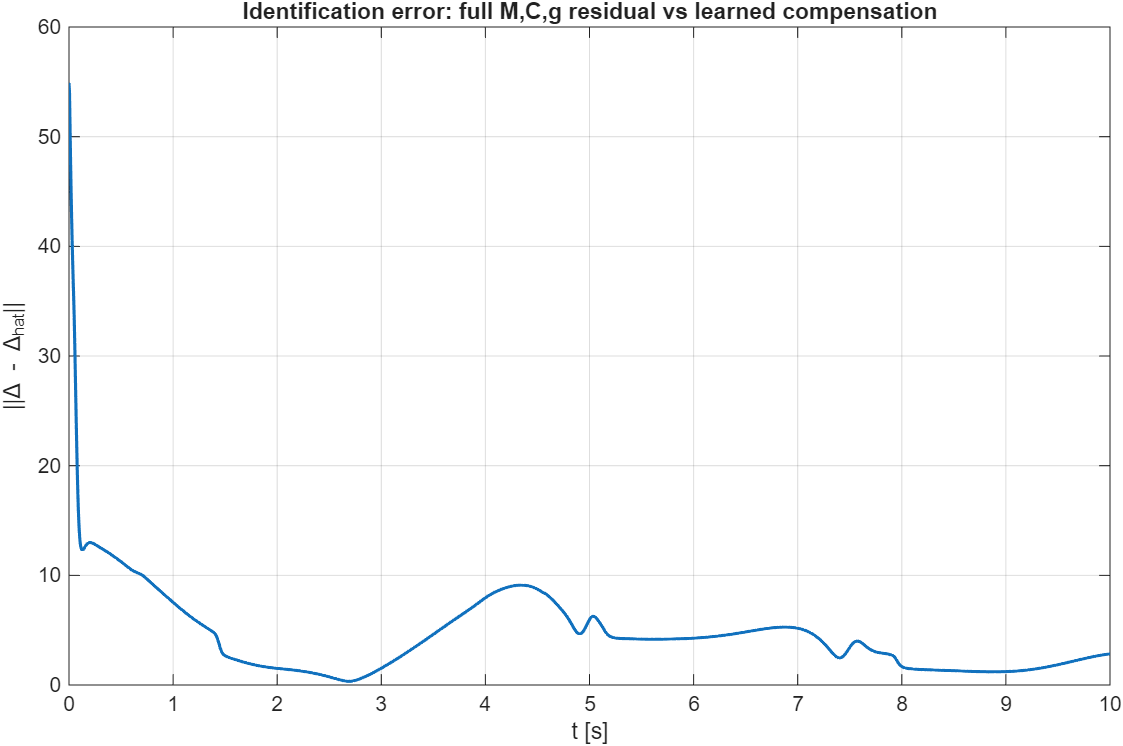
\includegraphics[width=\linewidth]{Images/learning_residual.png}
    \end{figure}
  \end{column}

  \begin{column}{0.31\textwidth}
    \begin{figure}[htbp]
      \centering
      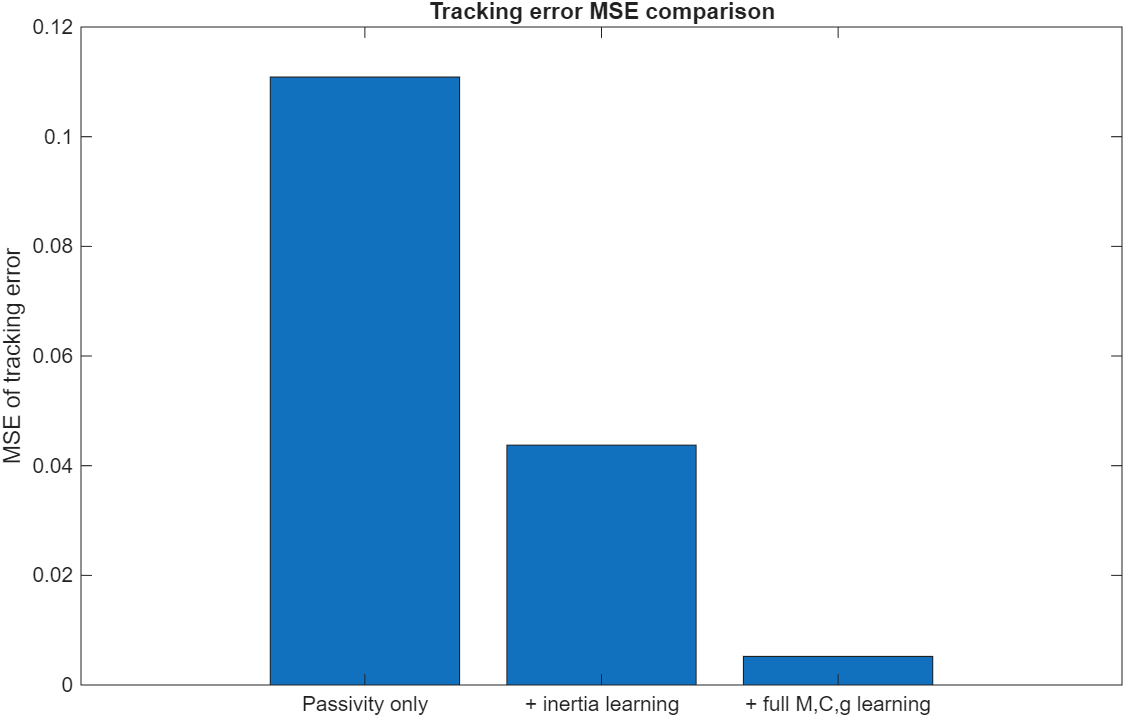
\includegraphics[width=\linewidth]{Images/MSE_comparison.png}
    \end{figure}
  \end{column}

    \begin{column}{0.31\textwidth}
    \begin{figure}[htbp]
      \centering
      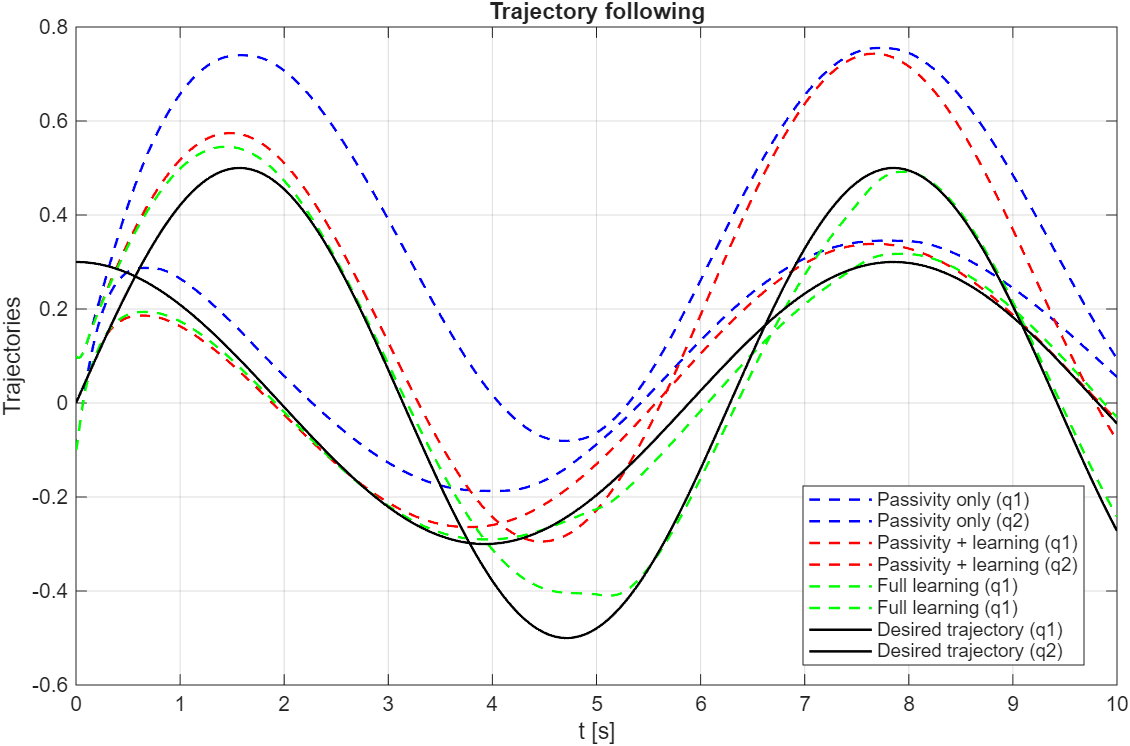
\includegraphics[width=\linewidth]{Images/Trajectories.png}
    \end{figure}
  \end{column}
\end{columns}\vspace{0.5cm}
Case with $20-40\%$ changes in mass, inertia and center-of-mass location, plus joint friction. The learning module reduces the residual $\tilde\Delta$ and the identification error $\|\tilde\Delta\|$.
\\ No offline training for the matrices, chosen at random, only online adaptation of the last layer. \end{frame}

%==================================================================
\section{Open points}
\begin{frame}{Open points and next steps}
\begin{enumerate}\setlength\itemsep{3pt}
\item \textbf{Offline training} of the DeLaN bases from momentum-window data (loop not yet implemented).
\item \textbf{Lipschitz/derivative certificate}: second-derivative bounds for Coriolis and gravity channels; choice of $\gamma$.
\item \textbf{STA gain conditions} under the $M^{-1}(q)$ coupling (Route 1 vs.\ Route 2).
\item Simulations: PBC only $\to$ full learning $\to$ full learning + STA.
\item Possible changes: IDA-PBC / port-Hamiltonian (regulation only; tracking and matched-uncertainty questions open); reservoir computing.
\end{enumerate}
\end{frame}

%==================================================================
\begin{frame}[allowframebreaks]{References}
\footnotesize
\setbeamertemplate{bibliography item}{}
\begin{thebibliography}{99}
\bibitem{sl87} J.-J.~E.~Slotine and W.~Li, ``On the adaptive control of robot manipulators,'' \emph{Int.\ J.\ Robotics Research}, 6(3):49--59, 1987.
\bibitem{os89} R.~Ortega and M.~W.~Spong, ``Adaptive motion control of rigid robots: a tutorial,'' \emph{Automatica}, 25(6):877--888, 1989.
\bibitem{biw91} C.~I.~Byrnes, A.~Isidori and J.~C.~Willems, ``Passivity, feedback equivalence, and the global stabilization of minimum phase nonlinear systems,'' \emph{IEEE TAC}, 36(11):1228--1240, 1991.
\bibitem{orte02} R.~Ortega, A.~van der Schaft, B.~Maschke and G.~Escobar, ``Interconnection and damping assignment passivity-based control of port-controlled Hamiltonian systems,'' \emph{Automatica}, 38(4):585--596, 2002.
\bibitem{br24} P.~Borja and R.~Ortega, \emph{Introduction to Passivity-based Control}, 2024.
\bibitem{lut19} M.~Lutter, K.~Listmann and J.~Peters, ``Deep Lagrangian networks for end-to-end learning of energy-based control for under-actuated systems,'' \emph{IROS}, 5562--5569, 2019.
\bibitem{shi19} G.~Shi et al., ``Neural Lander: stable drone landing control using learned dynamics,'' \emph{ICRA}, 2019.
\bibitem{miy18} T.~Miyato et al., ``Spectral normalization for generative adversarial networks,'' \emph{ICLR}, 2018.
\bibitem{dlm03} A.~De~Luca and R.~Mattone, ``Actuator failure detection and isolation using generalized momenta,'' \emph{ICRA}, 2003.
\bibitem{swe97} J.~Swevers et al., ``Optimal robot excitation and identification,'' \emph{IEEE Trans.\ Robotics and Automation}, 13(5):730--740, 1997.
\bibitem{mo12} J.~A.~Moreno and M.~Osorio, ``Strict Lyapunov functions for the super-twisting algorithm,'' \emph{IEEE TAC}, 57(4):1035--1040, 2012.
\bibitem{ut92} V.~I.~Utkin, \emph{Sliding Modes in Control and Optimization}, Springer, 1992.
\bibitem{is96} P.~A.~Ioannou and J.~Sun, \emph{Robust Adaptive Control}, Prentice Hall, 1996.
\bibitem{sp06} M.~W.~Spong, S.~Hutchinson and M.~Vidyasagar, \emph{Robot Modeling and Control}, Wiley, 2006.
\bibitem{kel05} R.~Kelly, V.~Santib\'a\~nez and A.~Lor\'ia, \emph{Control of Robot Manipulators in Joint Space}, Springer, 2005.
\bibitem{pog98} A.~Y.~Pogromsky, ``Passivity based design of synchronizing systems,'' \emph{Int.\ J.\ Bifurcation and Chaos}, 8(2):295--319, 1998.
\end{thebibliography}
\end{frame}

\end{document}
